\section{Relation to Prior Work}
\label{sec:relaltion}

In this section we relate relevant prior work on CGD algorithms for fitting AAMs \cite{Matthews2004, Gross2005, Papandreou2008, Amberg2009, Martins2010, Tzimiropoulos2013, Kossaifi2014} to the unified and complete view introduced in the previous Section.

\subsection{Project-Out algorithms}

In their seminal work \cite{Matthews2004}, Matthews and Baker proposed the first CGD algorithm for fitting AAMs, the so-called Project-out Inverse Compositional (PIC) algorithm. This algorithm uses Gauss-Newton to solve the optimization problem posed by the project-out cost function using inverse composition. The use of the project-out norm removes the need to solve for the appearance parameters and the use of inverse composition allows for the precomputation of the pseudo-inverse of the Jacobian with respect to $\Delta\mathbf{p}$, i.e. $\left( \mathbf{J}_{\bar{\mathbf{a}}}^T\bar{\mathbf{A}}\mathbf{J}_{\bar{\mathbf{a}}} \right)^{-1}\mathbf{J}_{\bar{\mathbf{a}}}\bar{\mathbf{A}}$. The PIC algorithm is very efficient ($O(nF)$) but it has been shown to perform poorly in generic and unconstrained scenarios \cite{Gross2005, Papandreou2008}. In this paper, we refer to this algorithm as the \emph{Project-Out Inverse Gauss-Newton} algorithm.

The forward version of the previous algorithm, i.e. the \emph{Project-Out Forward Gauss-Newton} algorithm, was initially proposed by Amberg et al. in \cite{Amberg2009} and reintroduced, under the name Fast-Forward, by Tzimiropoulos and Pantic in \cite{Tzimiropoulos2013}. In this case, the use of forward composition prevents the precomputation of the Jacobian pseudo-inverse and its asymptotic complexity increases to $O(nmF + n^2F + n^3)$. However, this algorithm has been shown to largely outperform its inverse counterpart, and obtains good performance under generic and unconstrained conditions \cite{Amberg2009, Tzimiropoulos2013}\footnote{Notice that, in \cite{Amberg2009}, Amberg et al. also introduced a hybrid forward/inverse algorithm, coined CoLiNe. This algorithm is a compromise between the previous two algorithms in terms of both complexity and accuracy. Due to its rather ad-hoc derivation, this algorithm was not considered in this paper.}

To the best of our knowledge, the rest of Project-Out algorithms derived in Section \ref{sec:fitting}, i.e.:
\begin{itemize}
\item \emph{Project-Out Asymmetric Gauss-Newton}
\item \emph{Project-Out Bidirectional Gauss-Newton Schur}
\item \emph{Project-Out Bidirectional Gauss-Newton Alternated}
\item \emph{Project-Out Forward Newton}
\item \emph{Project-Out Inverse Newton Schur}
\item \emph{Project-Out Asymmetric Newton}
\item \emph{Project-Out Bidirectional Newton Schur}
\item \emph{Project-Out Bidirectional Newton Alternated}
\end{itemize}
have never been published before and are a significant contribution of this work.

\subsection{SSD algorithms}

In \cite{Gross2005} Gross et al. presented the \emph{Simultaneous Inverse Compositional} (SIC) algorithm and show that it largely outperforms the \emph{Project-Out Inverse Gauss-Newton} algorithm in terms of fitting accuracy. This algorithm uses Gauss-Newton to solve the optimization problem posed by the SSD cost function using inverse composition. In this case, the Jacobian with respect to $\Delta\mathbf{p}$, depends on the current value of the appearance parameters and needs to be recomputed at every iteration. Moreover, the inclusion of the Jacobian with respect to the appearance increments $\delta\mathbf{c}$, increases the size of the simultaneous Jacobian to $\frac{\partial\mathbf{r}}{\partial\Delta\boldsymbol{\ell}} = \left( -\mathbf{A}, -\mathbf{J}_\mathbf{a} \right) \in R^{F \times (m + n)}$ and, consequently, the computational cost per iteration of the algorithm is $O((m + n)^2F + (m + n)^3)$.

As we shown in Sections \ref{sec:gauss_newton_simultaneous}, \ref{sec:gauss_newton_alternated} and \ref{sec:wiberg} the previous complexity can be dramatically reduce by taking advantage of the problem structure in order to derive more efficient and exact algorithm by:
\begin{inparaenum}[\itshape a\upshape)]
\item applying the Schur complement;
\item adopting an alternated optimization approach; or
\item or using the Wiberg method.
\end{inparaenum}
Papandreou and Maragos \cite{Papandreou2008} proposed an algorithm that is equivalent to the solution obtained by applying the Schur complement to the problem, as described in Section \ref{sec:gauss_newton_simultaneous}. The same algorithm was reintroduced in \cite{Tzimiropoulos2013} using a somehow ad-hoc derivation (reminiscent of the Wiberg method) under the name Fast-SIC. This algorithm has a computational cost per iteration of $O(nmF + n^2F + n^3)$. In this paper, following our unified view on CGD algorithm, we refer to the previous algorithm as the \emph{SSD Inverse Gauss-Newton Schur} algorithm. The alternated optimization approach was used in \cite{Tzimiropoulos2012} and \cite{Antonakos2014} with complexity $O(n^2F + n^3)$ per iteration. We refer to it as the \emph{SSD Inverse Gauss-Newton Alternated} algorithm.

On the other hand, the forward version of the previous algorithm i.e. the \emph{Simultaneous Forward Compositonal} (SFC) algorithm was first proposed by Martins et al. in \cite{Martins2010}\footnote{Note that Martins et al.  used an additive update rule for the shape parameters, $\mathbf{p}_o =  \mathbf{p} + \delta\mathbf{p}$, so strictly speaking they derived an additive version of the algorithm i.e the \emph{Simultaneous Forward Additive} (SFA) algorithm.}. In this case, the Jacobian with respect to $\delta\mathbf{p}$ depends on the current value of the shape parameters $\mathbf{p}$ through the warped image $\mathbf{i}[\mathbf{p}]$ and also needs to be recomputed at every iteration. Consequently, the complexity if the algorithm is the same as in the naive inverse approach of Gross et al. In this paper, we refer to this algorithm as the \emph{SSD Forward Gauss-Newton} algorithm. It is important to notice that Tzimiropoulos and Pantic \cite{Tzimiropoulos2013} derived a more efficient version of this algorithm ($O(nmF + n^2F + n^3)$) by applying the same derivation used to obtain their Fast-SIC algorithm. They showed that in the forward case their derivation removed the need to explicitly solve for the appearance parameters. Their algorithm is equivalent to the previous \emph{Project-Out Forward Gauss-Newton}.

\begin{figure*}[t!]
	\centering
	\begin{subfigure}{0.16\textwidth}
		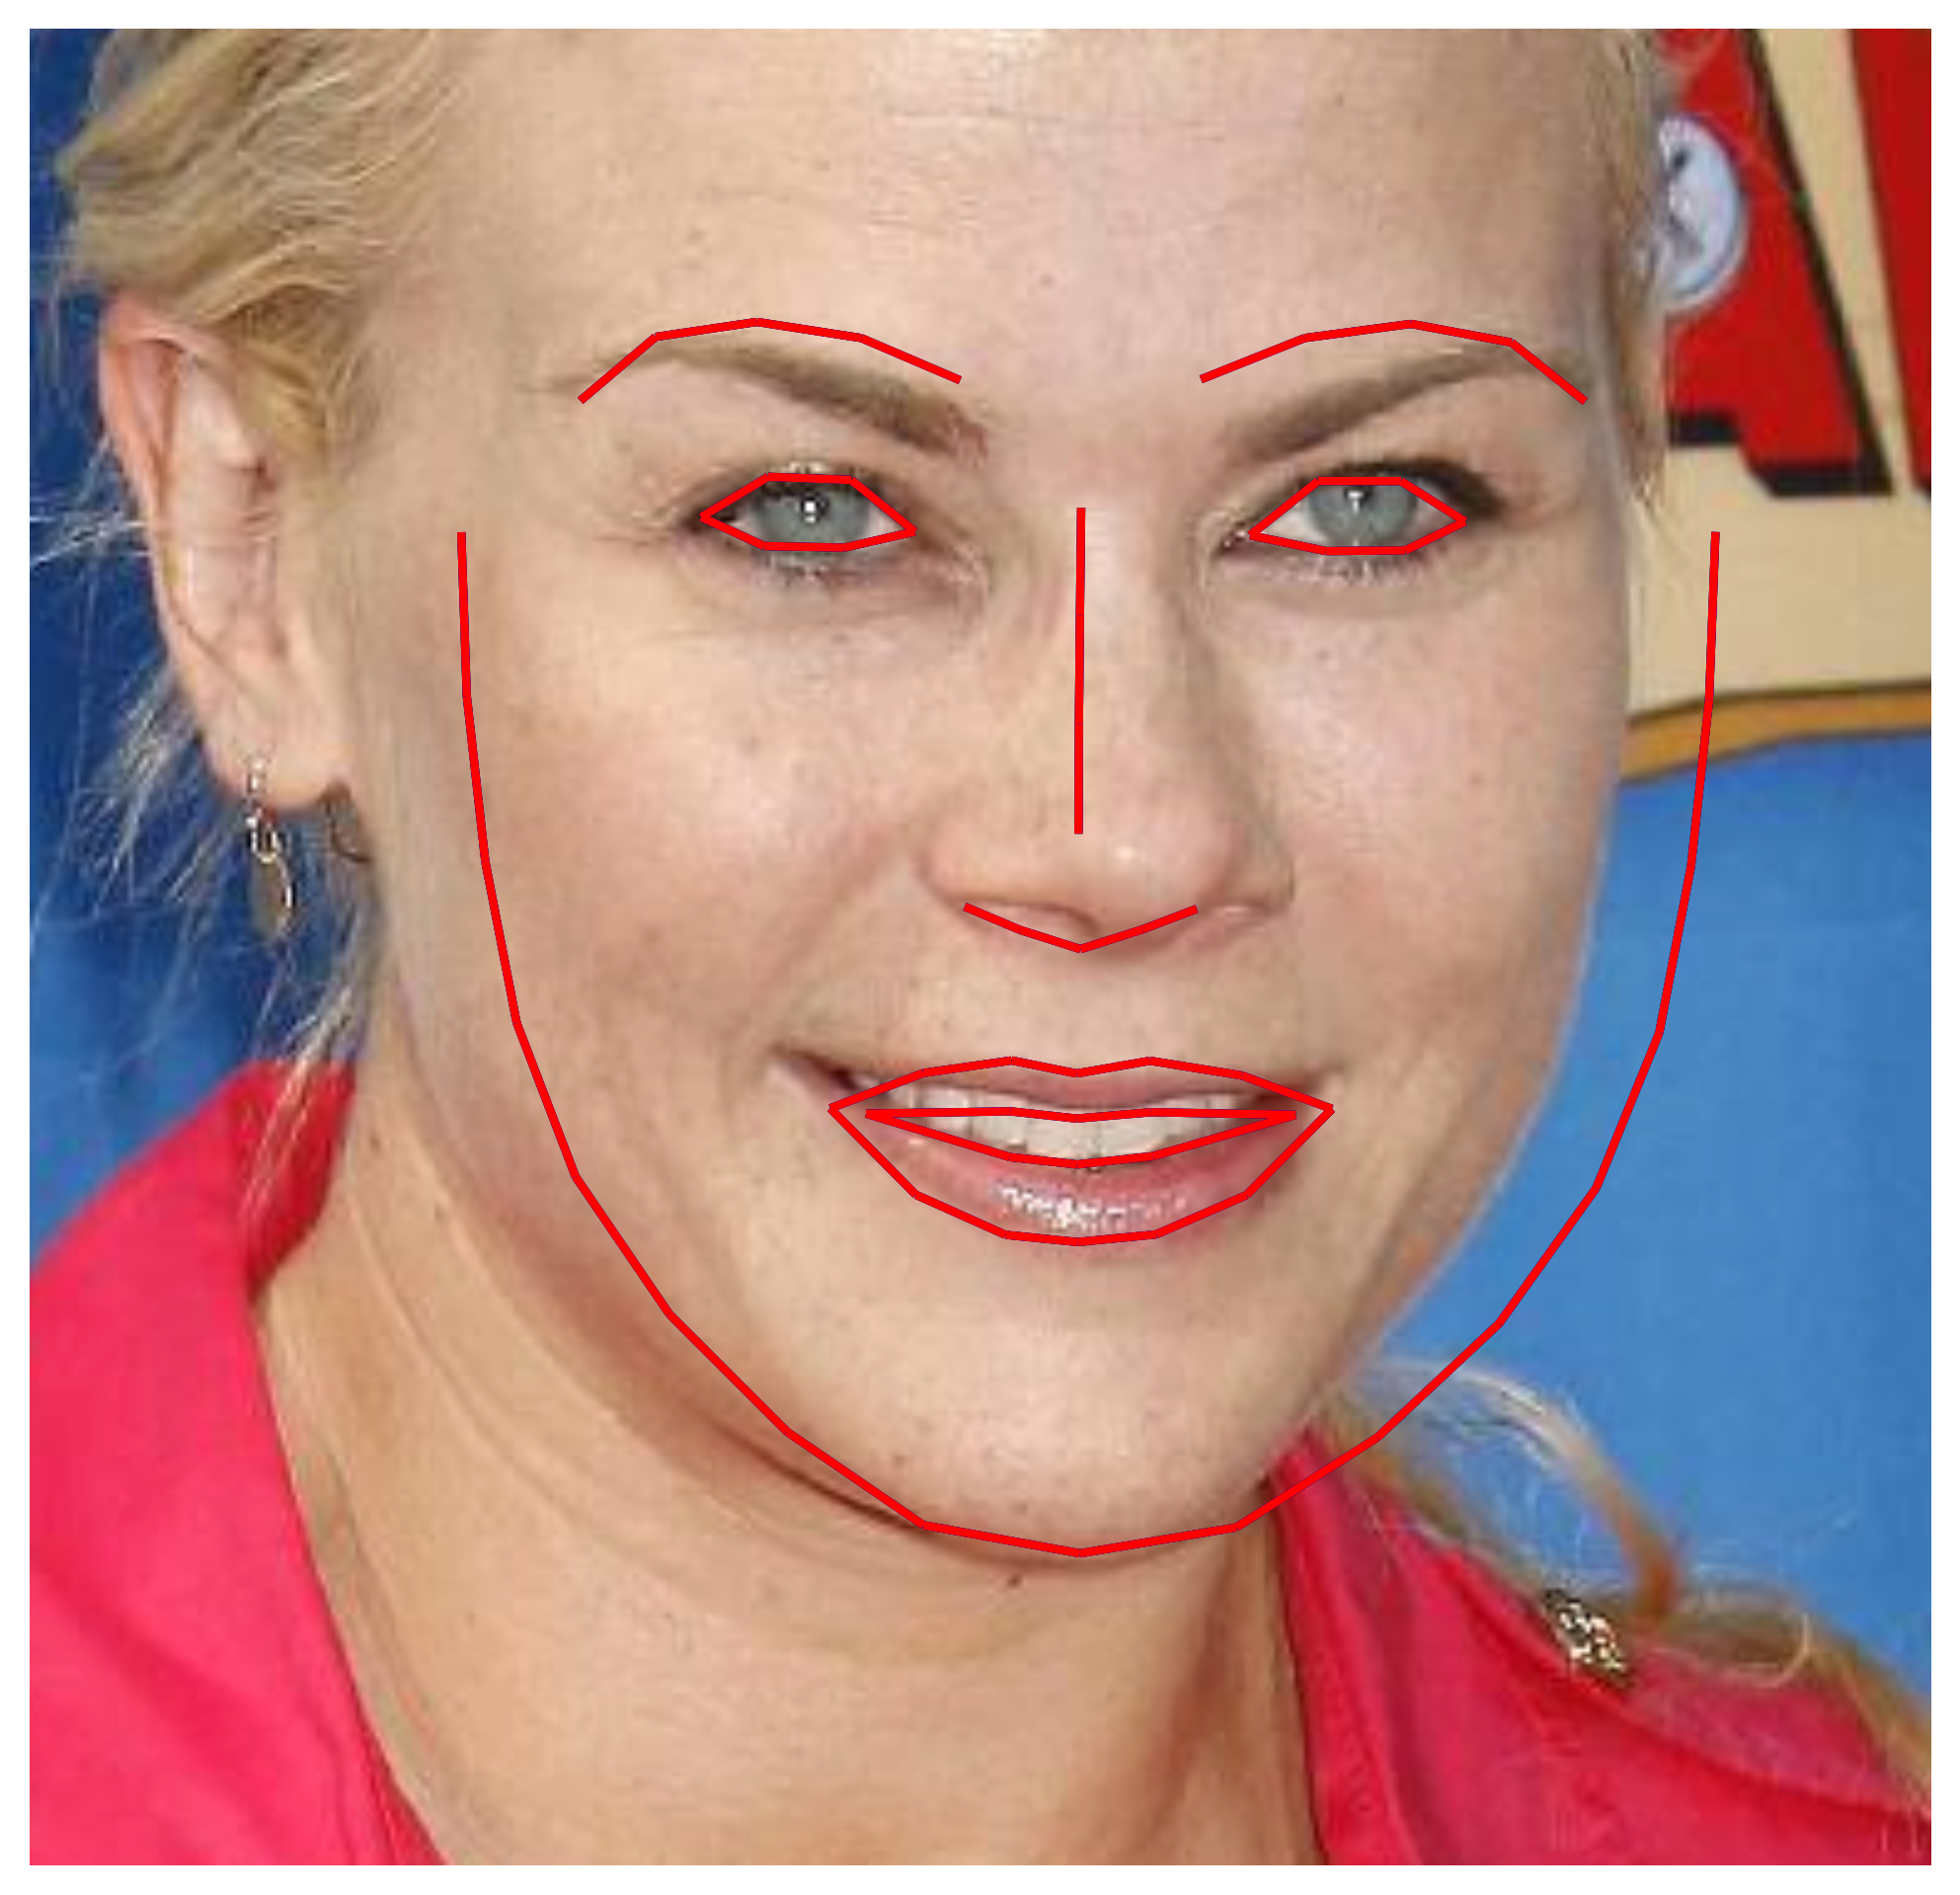
\includegraphics[width=\textwidth]{figures/ini_0.png}
		\caption{$0\%$}
		\label{fig:ini_0}
	\end{subfigure}
	\begin{subfigure}{0.16\textwidth}
		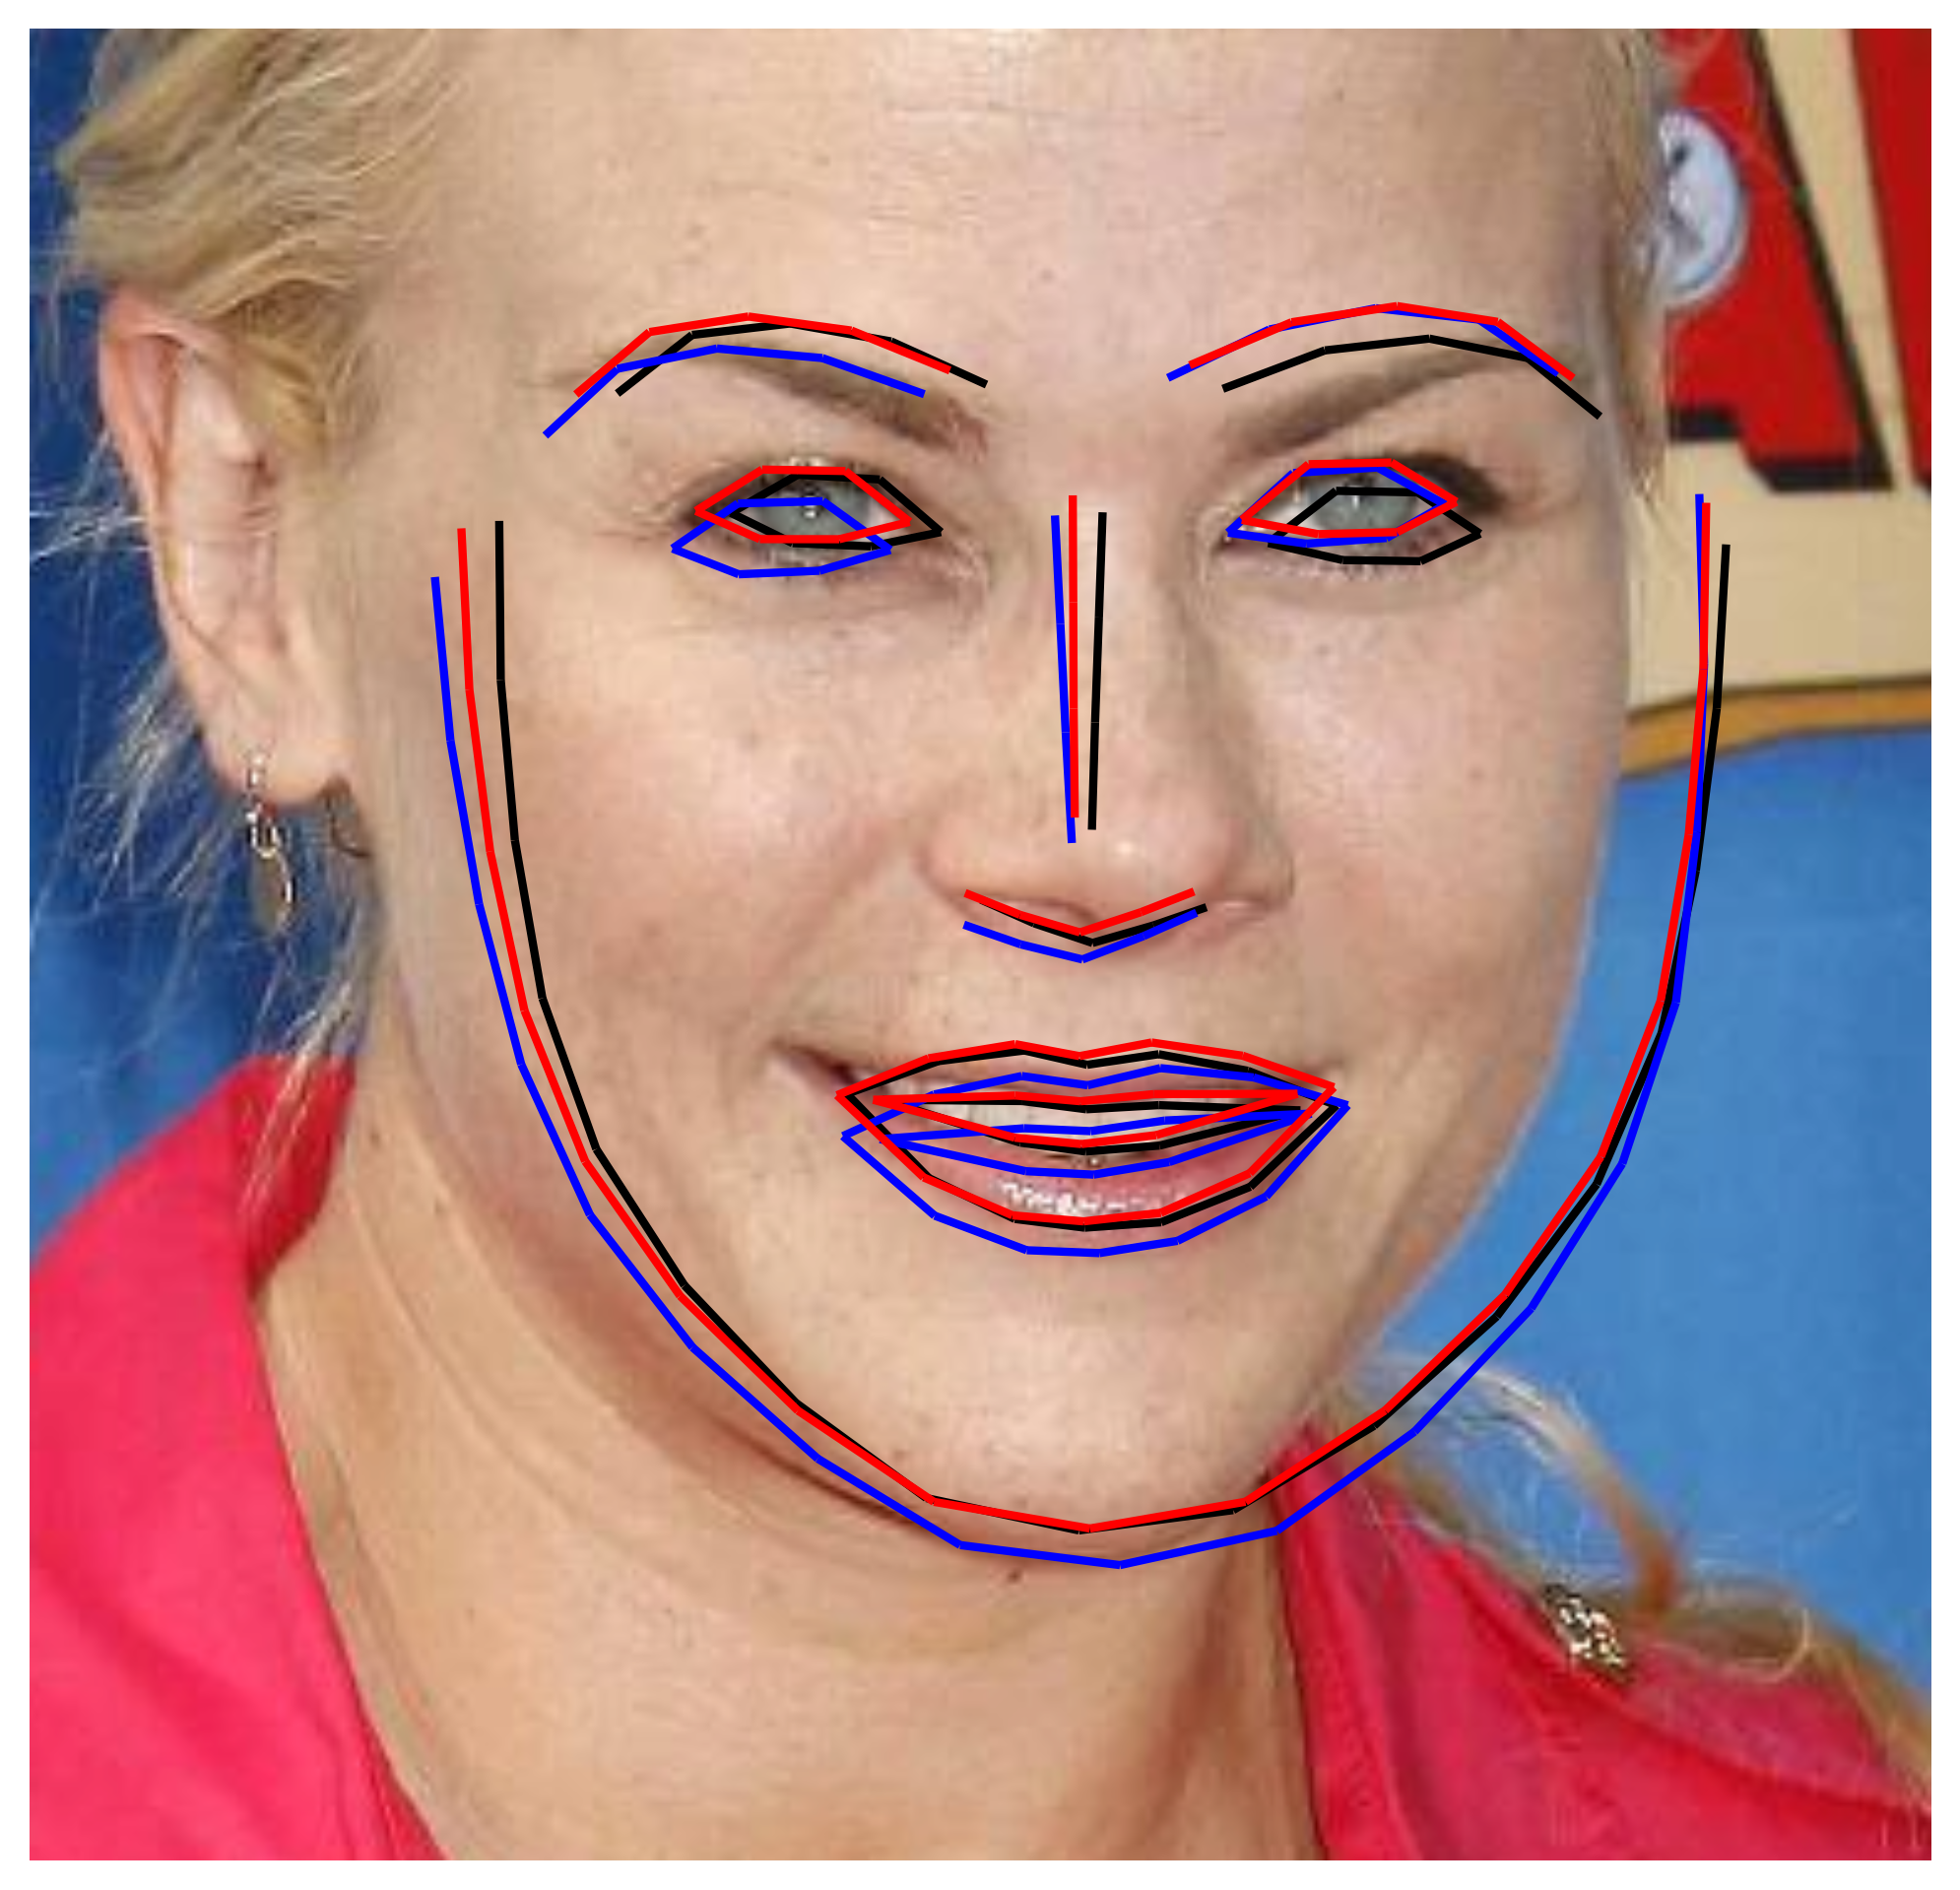
\includegraphics[width=\textwidth]{figures/ini_1.png}
		\caption{$2.5\%$}
		\label{fig:ini_1}
	\end{subfigure}
	\begin{subfigure}{0.16\textwidth}
		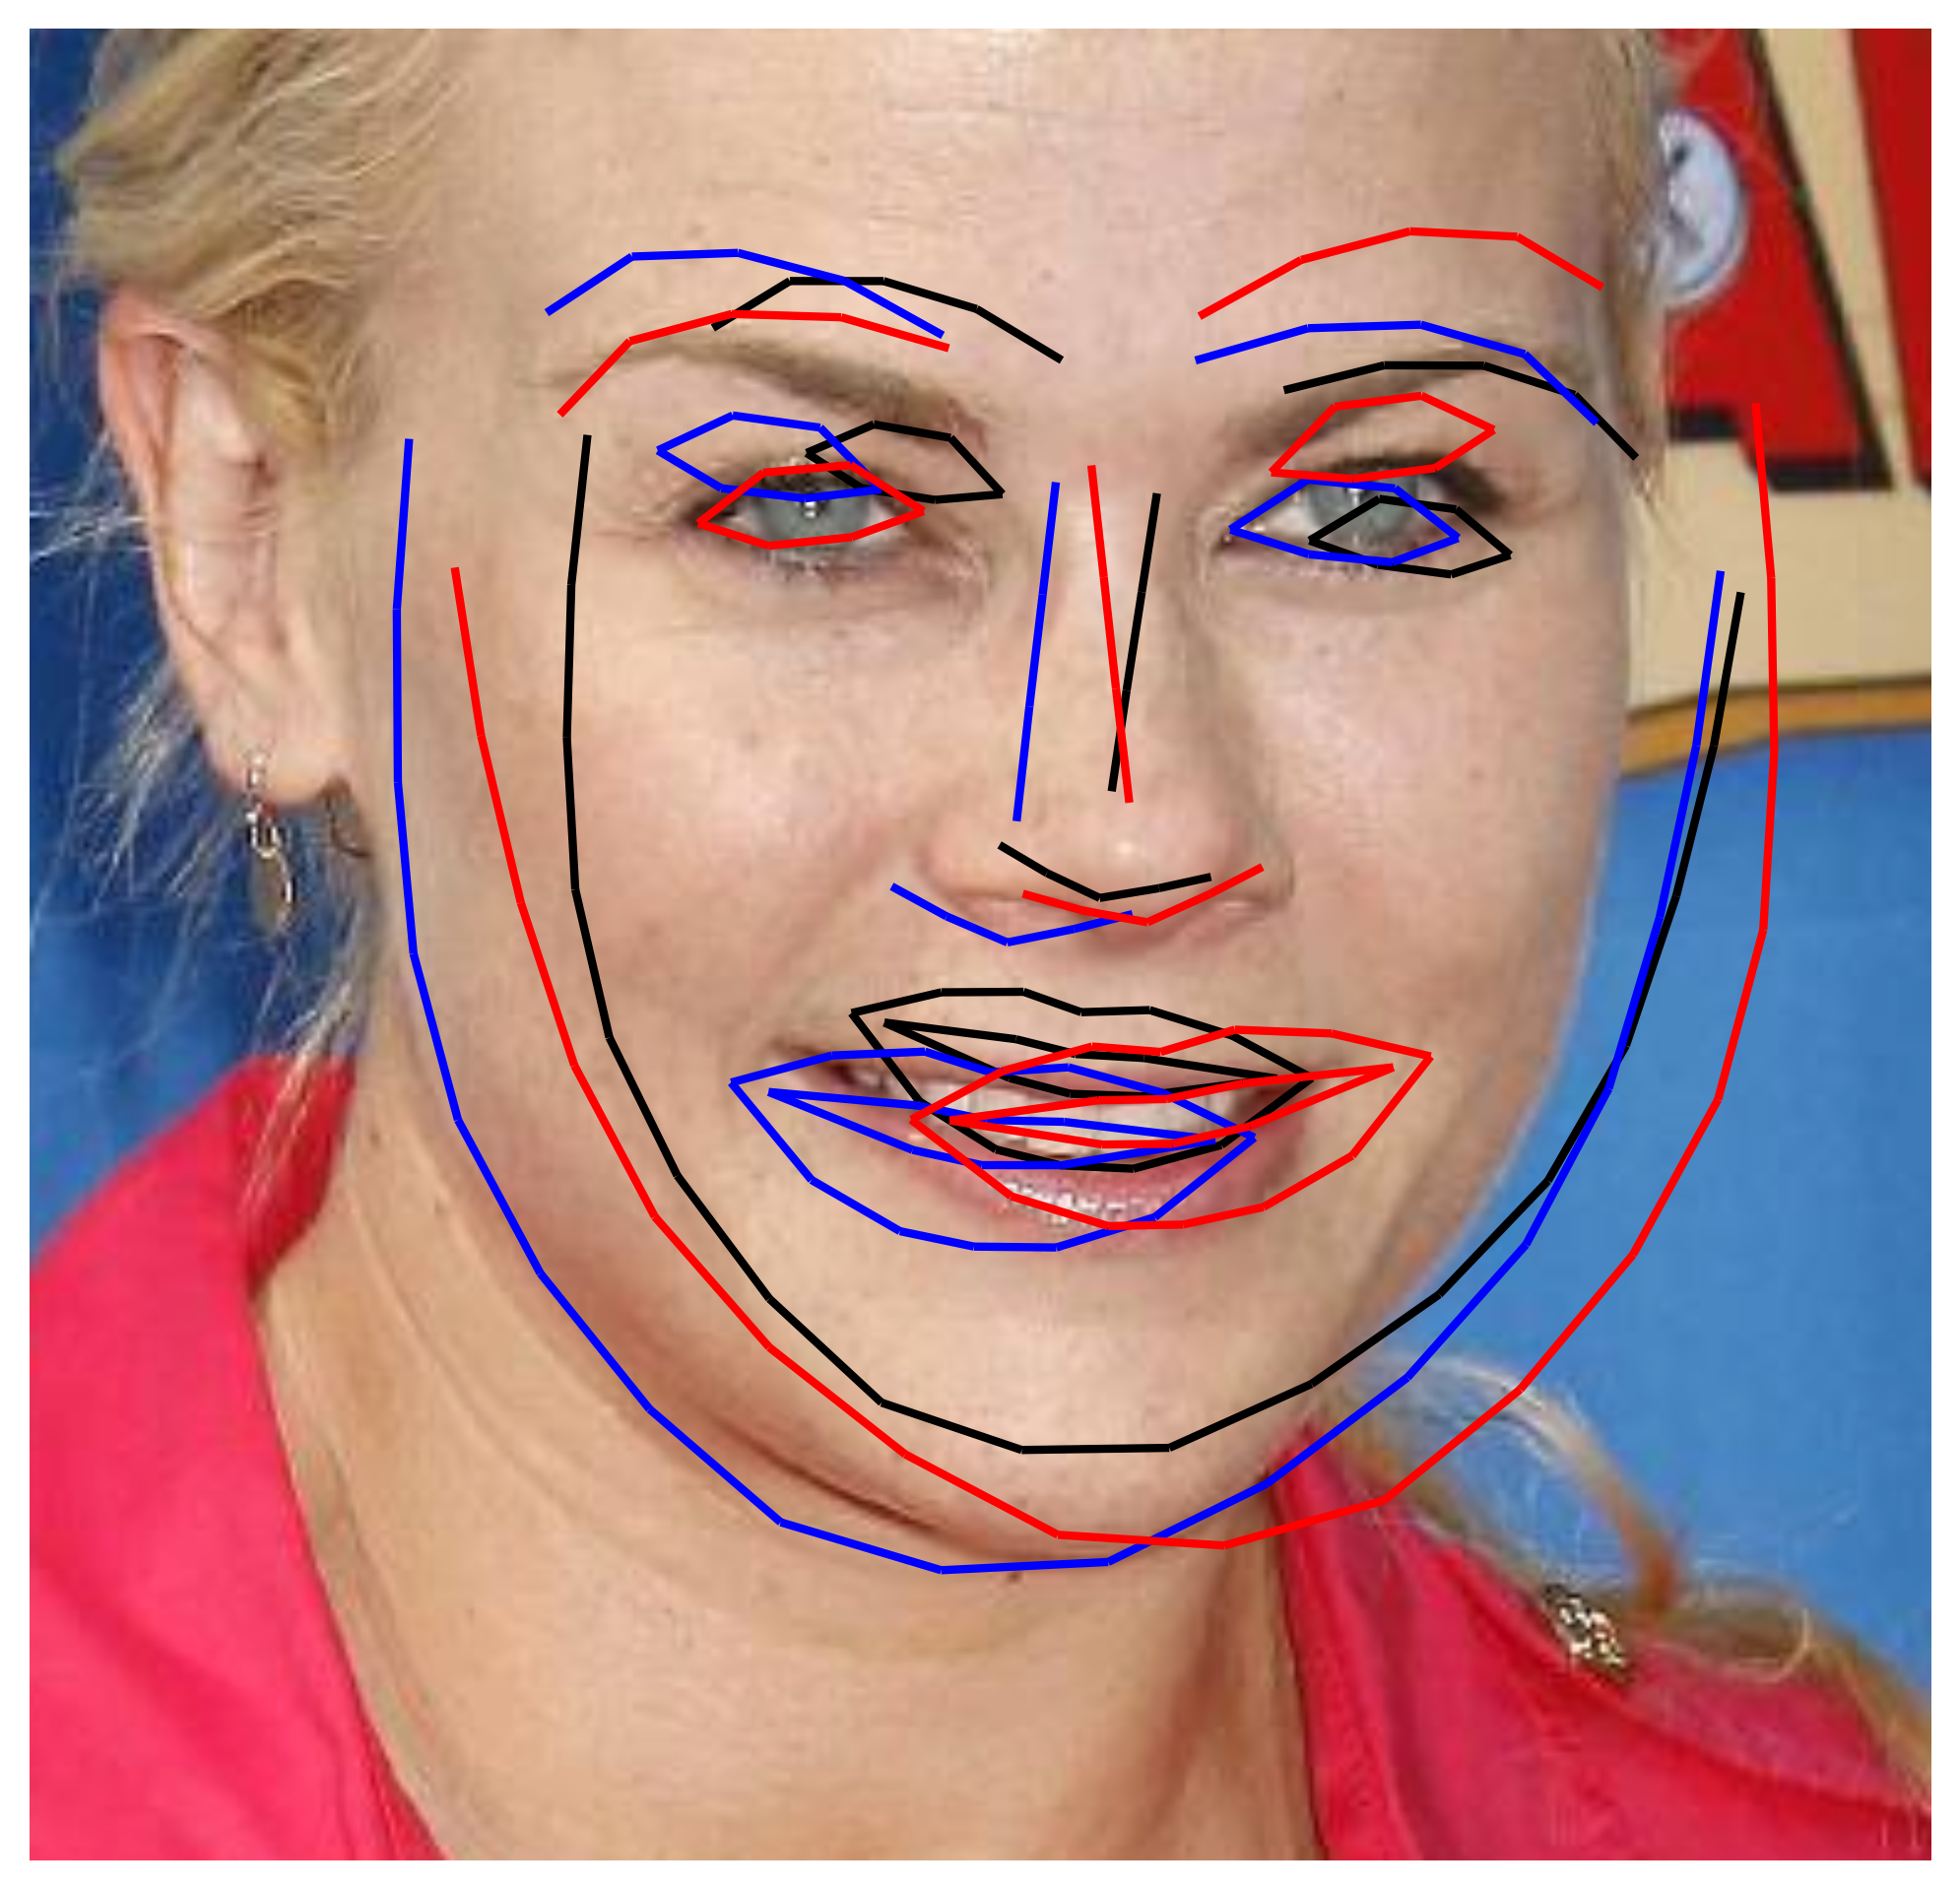
\includegraphics[width=\textwidth]{figures/ini_2.png}
		\caption{$5\%$}
		\label{fig:ini_2}
	\end{subfigure}
	\begin{subfigure}{0.16\textwidth}
		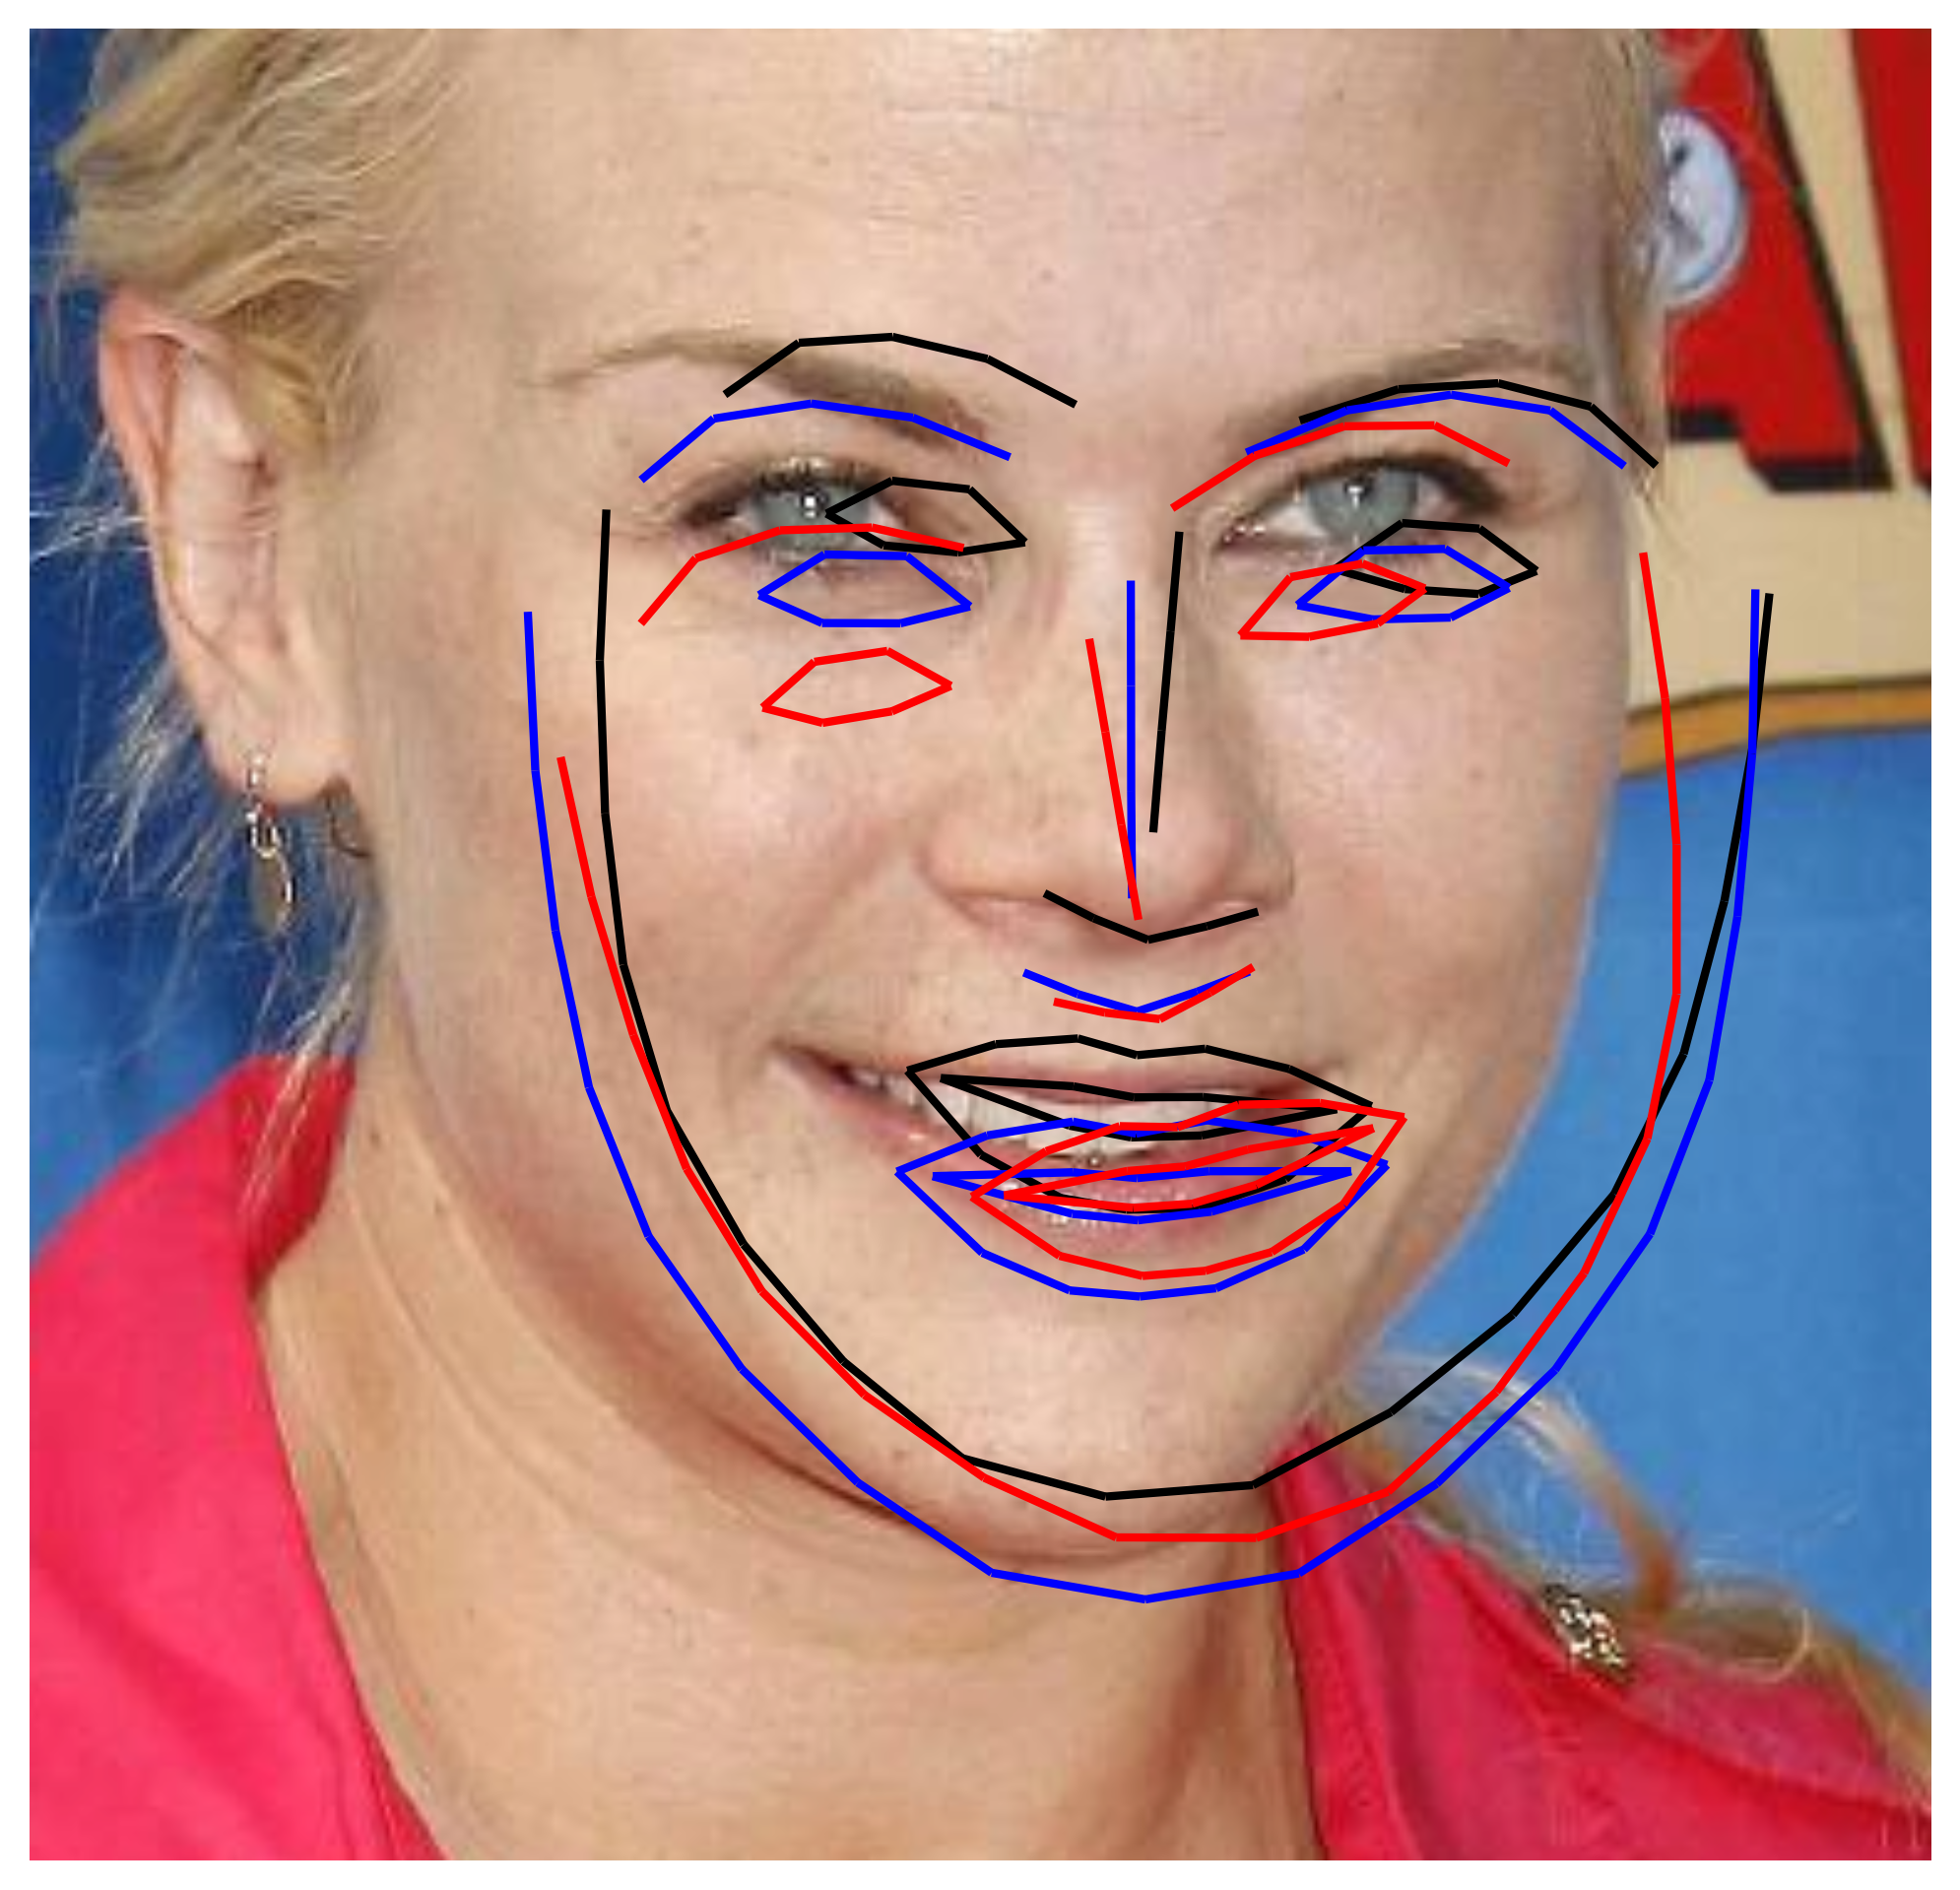
\includegraphics[width=\textwidth]{figures/ini_3.png}
		\caption{$7.5\%$}
		\label{fig:ini_3}
	\end{subfigure}
	\begin{subfigure}{0.16\textwidth}
		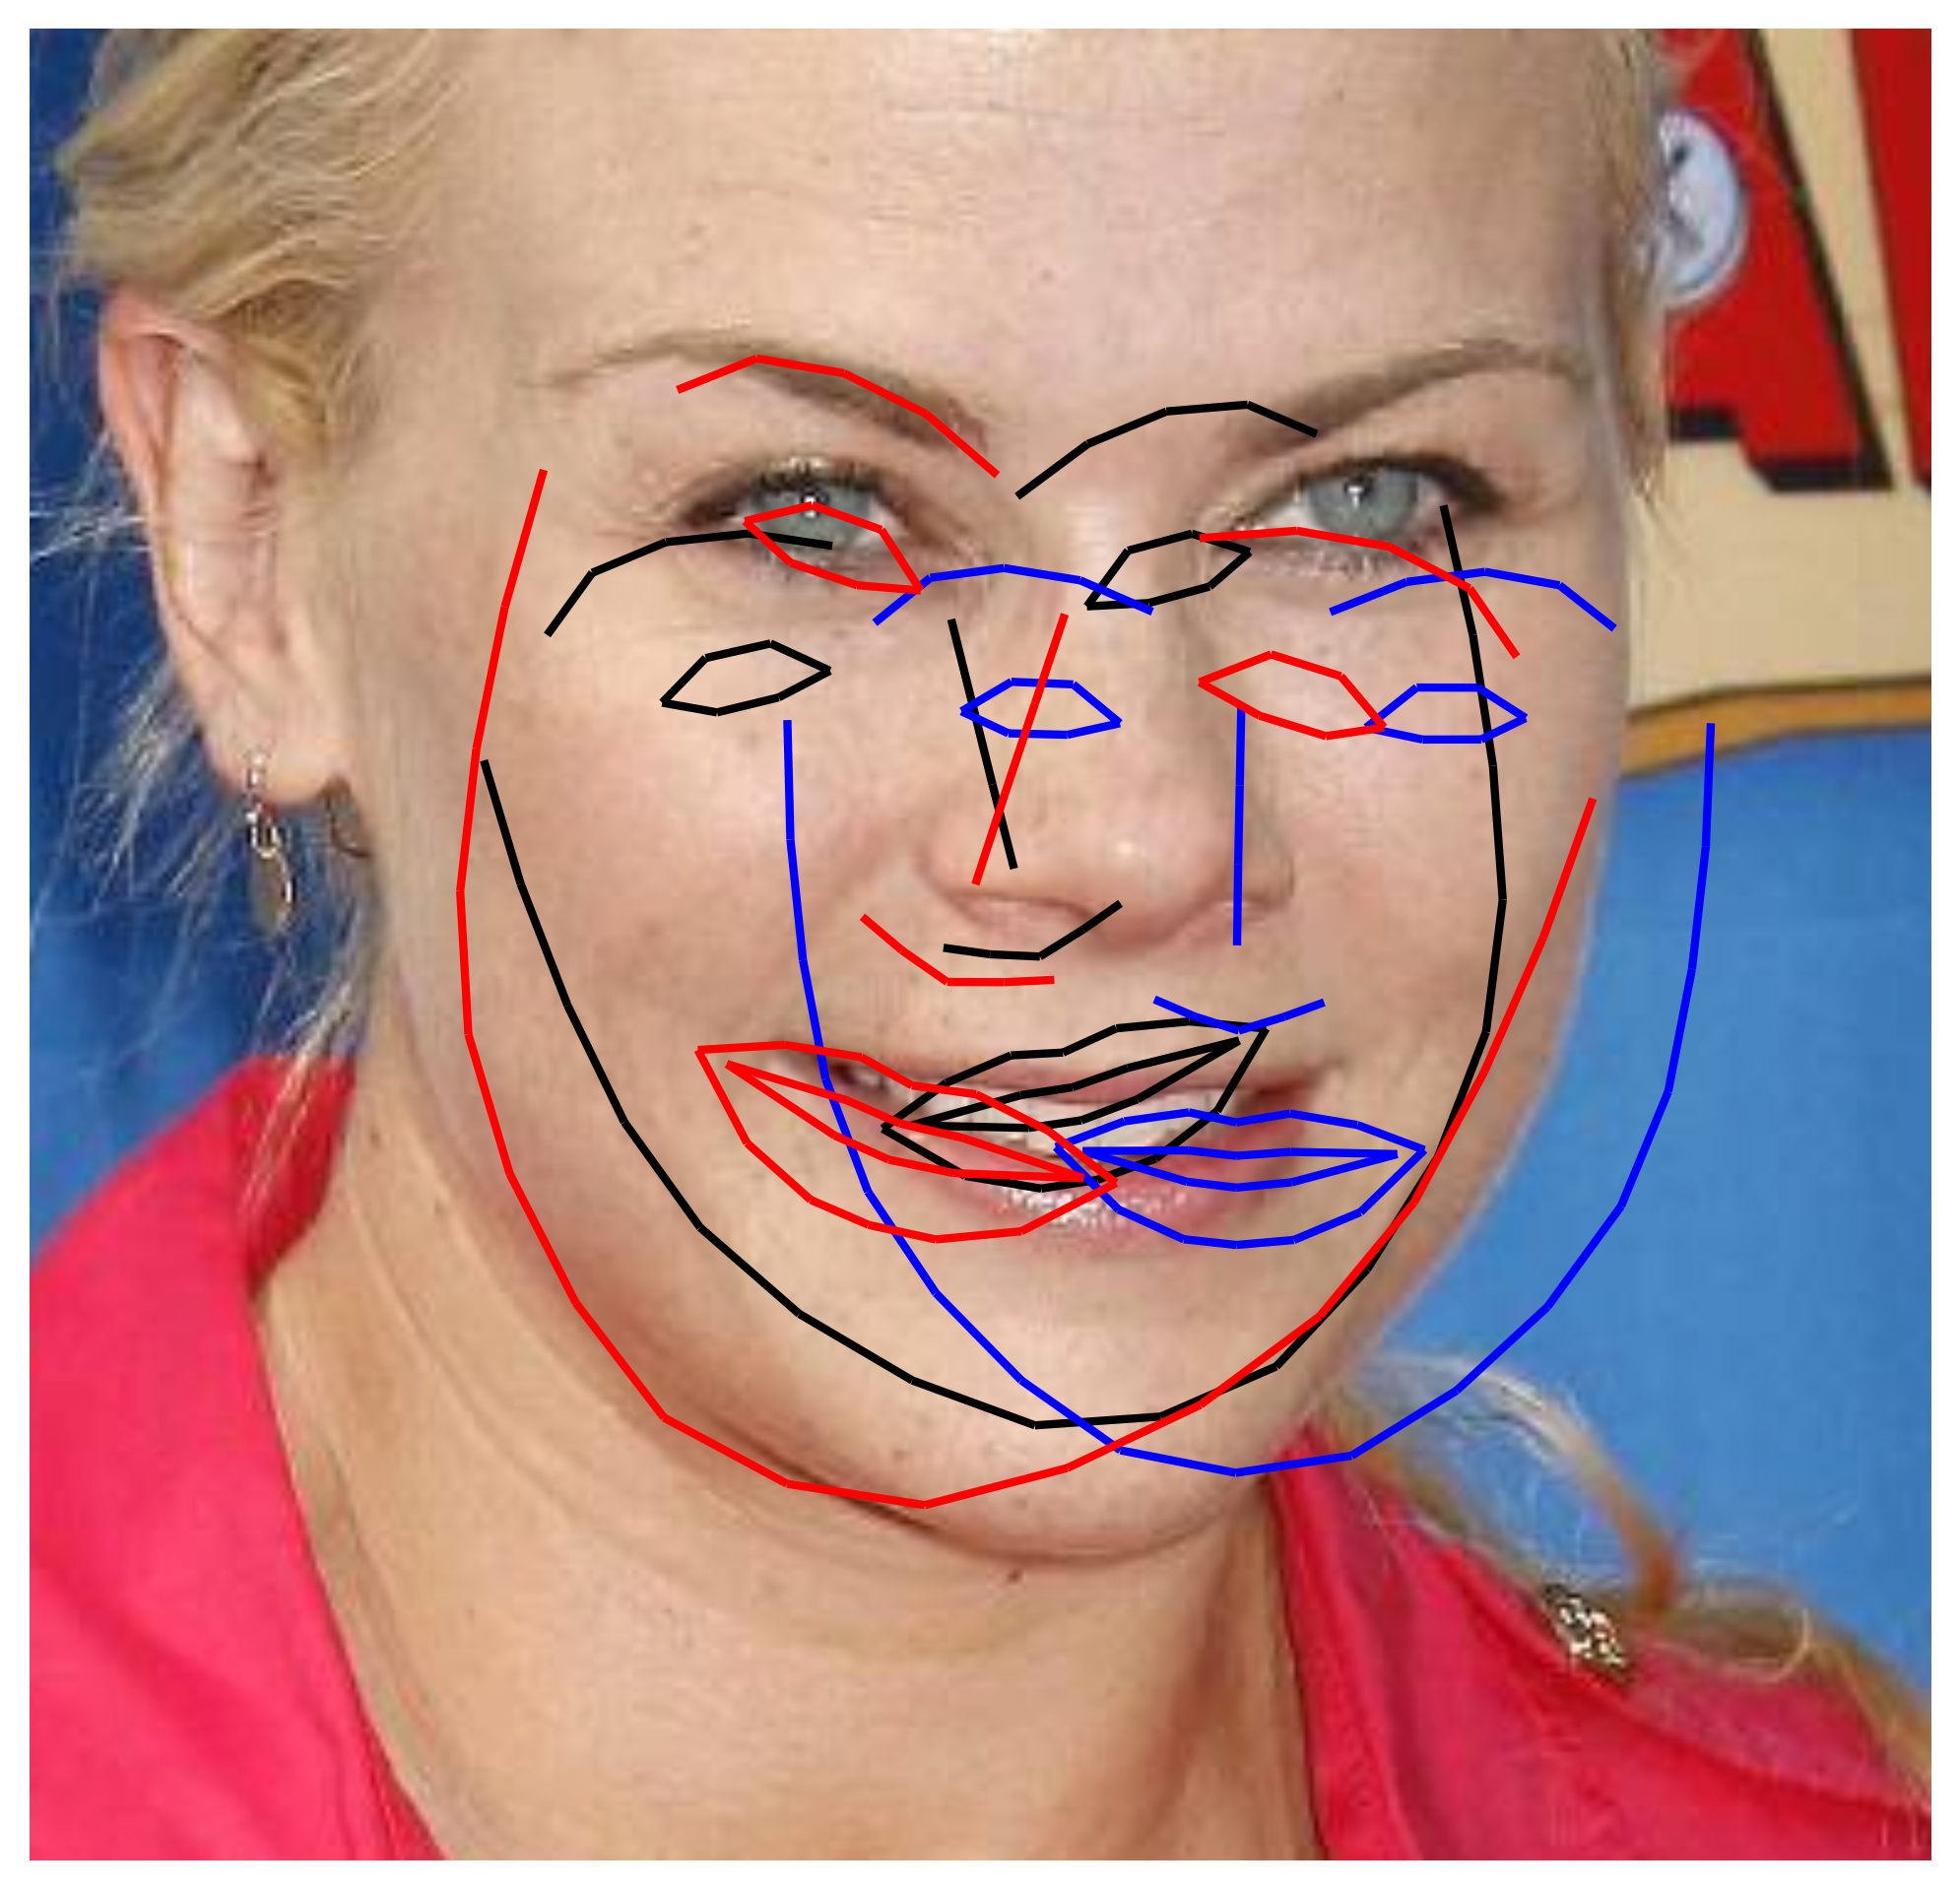
\includegraphics[width=\textwidth]{figures/ini_4.png}
		\caption{$10\%$}
		\label{fig:ini_4}
	\end{subfigure}
    \caption{Exemplar initializations obtained by varying the percentage of uniform noise added to the similarity parameters. Note that, increasing the percentage of noise produces more challenging initialization.}
    \label{fig:ini}
\end{figure*}

Finally, Kossaifi et al. derived the \emph{SSD Inverse Newton Schur} algorithm in \cite{Kossaifi2014}. This algorithm has a total complexity per iteration of $O(nmF + n^2m + 2n^2F + n^3)$ and was shown to slightly underperform its equivalent Gauss-Newton counterpart.

The remaining SSD algorithms derived in Section \ref{sec:fitting}, i.e.:
\begin{itemize}
\item \emph{SSD Forward Gauss-Newton Alternated}
\item \emph{SSD Asymmetric Gauss-Newton Schur}
\item \emph{SSD Asymmetric Gauss-Newton Alternated}
\item \emph{SSD Bidirectional Gauss-Newton Schur}
\item \emph{SSD Bidirectional Gauss-Newton Alternated}
\item \emph{SSD Forward Newton Schur}
\item \emph{SSD Forward Newton Alternated}
\item \emph{SSD Asymmetric Newton Schur}
\item \emph{SSD Asymmetric Newton Alternated}
\item \emph{SSD Bidirectional Newton Schur}
\item \emph{SSD Bidirectional Newton Alternated}
\end{itemize}
have never been published before and are also a key contribution of the presented work.